\documentclass{llncs}

\usepackage{graphicx}
%
\usepackage{geometry} % to change the page dimensions
\usepackage{multirow}
\usepackage{subfigure}


\geometry{a4paper}

\begin{document}


\title{Implementaci\'on de un Sistema Recuperaci\'on de Informaci\'on utilizando Redes Neuronales}

\author{Andy Gonz\'alez Pe\~na, Juan Eray \'Alvarez Hern\'andez}

\institute{MATCOM, Universidad de la Habana}
\maketitle


\begin{abstract}

Este trabajo recopila los puntos claves que conforman la implementaci\'on de un sistema de recuperaci\'on
de informaci\'on aunque no pretende proponer la mejor soluci\'on pero si una funcional para la aplicaci\'on
de los modelos de redes neuronales en la teor\'ia de los sistemas de recuperaci\'on de informaci\'on.

\end{abstract}

\section{Introducci\'on}\label{sec:Introduction}

Comenzaremos describiendo la estructura de la implementaci\'on, enumerando sus dependencias y definiendo la entrada y salida
del programa, con ello se va explicando su funcionamiento de manera general. \\
Luego para profundizar, subdividiremos las distintas tareas en cuatro  m\'odulos de los cuales se argumentan, de igual manera, su
funcionamiento y estructura demostrando el cumplimiento de los puntos requeridos en cada uno de ellos.\\
Finalmente, se enumeran ejemplos de acuerdo con los resultados obtenidos que muestran los puntos fuertes y d\'ebiles de la
implementaci\'on con el prop\'osito de darle continuidad al proceso de refinamiento en el que actualmente se encuentra.\\

\section{Estructura}\label{sec:Structure}

El proyecto se prefiere ver como un todo y aun as\'i consta de cuatro m\'odulos: interfaz de usuario, procesamiento de texto,
\'indice y modelado, todos implementados utilizando {\textit{Python}} (v3.6) con entradas y salidas sobre documentos de tipo
 {\textit{JSON}} que definen su comportamiento en cada instancia de la ejecuci\'on. \\
Cada m\'odulo existe en proceso diferente del sistema operativo y, \'unicamente, se relacionan mediante accesos al disco duro
para consultar los archivos de entrada y salida, para ello se cre\'o un sistema de notificaciones.\\
Todo fichero {\textit{JSON}}, como es conocido, son b\'asicamente diccionarios de llave-valor, entonces cada m\'odulo cuando
emita una salida escribir\'a la estampilla de tiempo que le corresponde logrando de esta forma que el m\'odulo que utilice ese
fichero como entrada sepa que ha ocurrido un cambio al mismo y sea capaz entonces de efectuar sus operaciones.\\
El orden de la comunicaci\'on es definido seg\'un su necesidad, en primera instancia se encuentra el m\'odulo de la interfaz de
usuario que emite como salida la propia entrada del m\'odulo de modelado y espera como entrada la salida del mismo. Mientras
los m\'odulos de procesamiento de textos e indizado se comportan de igual manera para la modelaci\'on no se comporta as\'i
como en un proceso plano, sino que se divide en tres instancias enviando y recibiendo de los otros m\'odulos hasta que logra
emitir la salida concisa que fue requerida por la interfaz de usuario. \\
En las secciones correspondientes a cada uno de ellos se discutir\'an los aspectos de su implementaci\'on y se definir\'an, de 
manera expl\'icita como se comportan para emitir una salida de datos consecuente a su situaci\'on.\\
Mientras, de manera general, se define la arquitectura del software seg\'un la interrelaci\'on existente presente en cada par
como indica siguiente figura.\\

{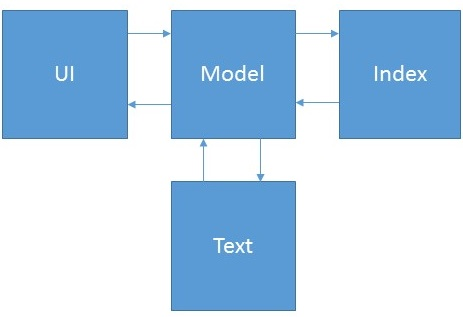
\includegraphics[]{structure}}
{\hfil\flushright{\textit{Fig 1. Interrelaci\'on de los m\'odulos}}}

\subsection{M\'odulo Interfaz de Usuario}

Es una interfaz web minimalista que cumple con los est\'andares de dise\~no para el cual el usuario solamente podr\'a interactuar
seg\'un el sistema indique.

\subsubsection{Dependencias}

Creada en {\textit{Python}} utilizando {\textit{Flask}} como {\textit{framework}} en el que las plantillas renderizadas deber\'an 
ser interpretadas debido al uso de {\textit{cookies}} en su definici\'on, entonces se requiere del m\'odulo denominado {\textit{jinja}}
para que act\'ue como int\'erprete.\\
Mientras, el dise\~no visual utiliza las clases definidas en {\textit{Bootstrap}} y los {\textit{scripts}} correspondientes, donde a
ellos se le ha a\~nadido uno propio para definir un reloj en la esquina superior derecha que ayuda a visualizar el tiempo transcurrido
entre procesos.

\subsubsection{Estructura}

Consta de cuatro rutas solamente y un enlace externo. En la barra de navegaci\'on al tope de la p\'agina est\'an enumeradas. Estas
son: ruta ra\'iz que, en caso de ser iniciada la aplicaci\'on, iniciar\'ar las {\textit{cookies}} y otras variables necesarias para la aplicaci\'on,
y en otro caso, simplemente redireccionar\'a hacia la ruta {\textbf{index}}, en ella se encuentra el grueso de la aplicaci\'on de lo cual
hablaremos a continuaci\'on, otra ruta es el "acerca" del proyecto, en el se encontrar\'an documentos relacionados con el tema como este
y, por \'ultimo, la ruta de evaluaci\'on del sistema en el que se ha descrito casos de prueba con las medidas definidas seg\'un la teor\'ia.

\subsubsection{Funcionamiento}

En la p\'agina principal se encontrar\'an los botones que indican las posibles opciones, es decir, si por ejemplo, a\'un no se ha construido
un modelo, solamente se podr\'a esperar una direcci\'on del sistema de archivos para construir uno y entonces si ya existe, se podr\'a
realizar una consulta.\\
Cada bot\'on funciona seg\'un su nombre lo indica, pero dos de ellos destacan por encima de todos ya que en ellos es donde se define
la salida v\'ia {\textit{JSON}} del sistema, los botones de construcci\'on y consulta se definen como indica la siguiente figura.

{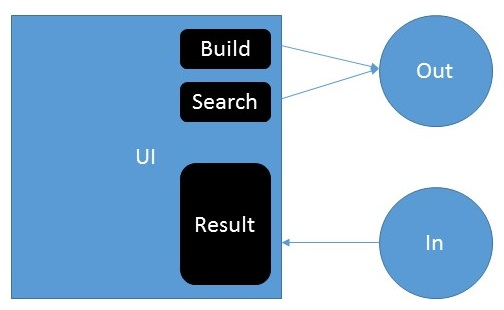
\includegraphics[]{ui}}
{\hfil\flushright{\textit{Fig 2. Entrada y salida de la interfaz de usuario}}}

\subsection{M\'odulo Procesamiento de Texto}

M\'odulo sencillo que recibe texto plano y realiza las operaciones requeridas para devolver una lista de t\'erminos v\'alidos para,
posteriormente, ser indizados.

\subsubsection{Metas alcanzadas}
El m\'odulo realiza las operaciones requeridas para el procesamiento de texto. Estas son: {\textit{stemming}} y la eliminaci\'on 
de {\textit{stopwords}} y se logran con la aplicaci\'on de la librer\'ia especificada en la secci\'on de dependencias.

\subsubsection{Dependencias}
Creada en {\textit{Python}} se apoya en su m\'odulo {\textit{NLTK}} que significa {\textit{Natural Language ToolKit}} especializado
en el procesamiento de lenguaje natural y, por consecuencia de texto, en \'el se encuentran distintos subm\'odulos, entre ellos los
necesarios son: {\textit{corpus}} y {\textit{stem}}.

\subsection{M\'odulo de Modelado}

Es el encargado de controlar el tr\'afico de datos necesarios para su computaci\'on. En primera instancia, hacia el m\'odulo de procesamiento
de texto realiza la conversi\'on de contenidos de ficheros a texto plano o una simple cadena de caracteres. Al tener la lista de todos los t\'erminos
a indizar los vectoriza en valores entre 0 y 1 y construye el modelo de redes neuronales.\\
Se define una red neuronal como una lista de matrices de pesos que representan las aristas entre nodos de capas adyacentes. Como prop\'osito
de generalizaci\'on, como se ver\'a adelante, se definen cuatro capas como se indica en la siguiente figura.

{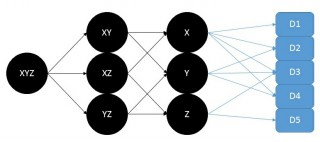
\includegraphics[]{model}}
{\hfil\flushright{\textit{Fig 3. Ejemplo de definici\'on del modelo}}}

En el vector de la capa de entrada est\'an los posibles t\'erminos de consulta, esos son todos los posibles t\'erminos a indizar y en el vector de la
capa de salida se encuentran los documentos posibles. Entonces para el momento de creaci\'on las matrices de pesos constar\'an de vectores
normalizados de n\'umeros aleatorios y se mantiene, adem\'as, los valores reales de {\textit{tf}} e {\textit{idf}} que ser\'an utilizados para 
obtener relaciones de pesos de aristas m\'as exactas.\\
Una vez finalizada la creaci\'on del modelo tambi\'en cumplir\'a con funciones vitales para el m\'odulo de \'indices, como por ejemplo, la consulta
no se realiza directamente del t\'ermino sino que se hace una conversi\'on de este hacia un vector de 0 y 1 que indican si la palabra existe en dicha
consulta o no. Este vector ser\'a el par\'ametro de entrada de la red neuronal.\\
Finalmente, el modelo est\'a implementado de tal forma que desde el punto de vista de la interfaz de usuario es un proceso unitario, es decir, en un ciclo de
ejecuci\'on obtiene su entrada, env\'ia y recibe lo necesario de los siguientes m\'odulos, primero procesa textos, luego crea o busca \'indices y,
finalmente, emite su salida hacia la interfaz. Esto significa que su apariencia es la siguiente:

{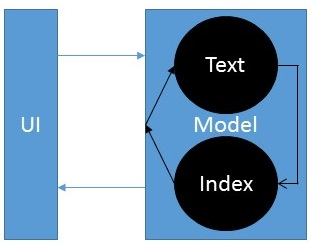
\includegraphics[]{appereance}}
{\hfil\flushright{\textit{Fig 4. Apariencia en ejecuci\'on del modelo}}}


\subsection{M\'odulo de \'Indices}

Este modelo tiene dos instancias fundamentales, cuando le es encomendada la tarea de finalizar la creaci\'on del modelo y cuando se realiza una consulta.
Se les dice fundamentales ya que el resto depende directamente del funcionamiento de estas dos.\\
Cuando construye la red neuronal se tiene la matriz de pesos descrita en la secci\'on anterior y se tienen los valores de {\textit{tf}} e {\textit{idf}},
entonces se quiere buscar la convergencia de la red, es decir, que dada una consulta sea capaz de retornar la probabilidad de relevancia a un documento.
Es, de tal forma, que se asume que los pesos aleatorios predefinidos no son buenos valores para tal objetivo, entonces dados los otros dos par\'ametros
del m\'odulo, se obtendr\'an la relevancia sobre los documentos, por tanto, para toda consulta unitaria, es decir, el vector de entrada que contiene solo
un 1 y el resto 0, se conocen sus valores de salida y se comienza la evaluaci\'on de nuestra red.\\
Se realiza el algoritmo hacia adelante, se eval\'ua el error y de acuerdo a la direcci\'on del gradiente negativo se recalculan los pesos y se propaga el error
en la red. Es importante destacar que la funci\'on de activaci\'on utilizada es la sigmoidal, tal que su derivada es la utilizada para la propagaci\'on. Esta es:\\
${\Delta}w{^{(t+1)}}_{i,j} = lrate * Err_{j} * o_j * (1 - o_j) * o_i$\\
Luego de evaluar un n\'umero finito de iteraciones, se establece el modelo de redes neuronales y permite analizar consultas. Para este caso, no se calcula
el error y se propaga para dar mejores resultados, sino que de manera directa se corre el algoritmo hacia adelante y se emite una salida.\\
Las salidas del m\'odulo son vectores de n\'umeros entre 0 y 1, que representan la activaci\'on del documento con respecto a la consulta. Posteriormente,
estas son procesadas y englobadas con los datos requeridos a la salida real del sistema como puede ser el nombre del documento.

\subsubsection{Limitaciones}
El costo en memoria depende directamente de la cantidad de t\'erminos a indizar, ya que las matrices tienen medidas variables respecto a ello por ende
para un gran n\'umero de t\'erminos puede ser altamente costoso y no solo en memoria ya que las multiplicaciones matriciales conllevan un gran uso de 
CPU y por tanto, de tiempo computacional.

\subsubsection{Dependencias}

Creada en {\textit{Python}} no tiene ning\'un requerimento especial.

\section{Conclusiones}
Un n\'umero estratosf\'erico de aplicaciones tienen las redes neuronales y constantemente se suman nuevas. Mientras, de manera rudimentaria, creamos
nuestra primera red neuronal con la cual obtenemos resultados satisfactorios. Se ha comprobado la teor\'a del \'algebra lineal aplicada a este modelo y su
similaridad con el modelo vectorial para inicializar sus valores de c\'omputo, adem\'as de la raz\'on por la cual es llamada un paradigma propio dentro de la
teor\'ia de la recuperaci\'on de informaci\'on.\\
Es importante destacar que este trabajo no termina a\'un, ya que como meta inmediata se encuentran temas como la retroalimentaci\'on dada las consultas
para extender su propia definici\'on de red neuronal.\\
En conjunto a la evaluaci\'on se ha comprobado que para mayores cantidades de t\'erminos y documentos el sistema obtiene mejores resultados en cuanto a
su exactitud, y por tanto para valores peque\~nos es m\'as propenso a retornar documentos que no son relevantes dada cualquier consulta.\\

\begin{thebibliography}{1}

\bibitem{data}
Grus, J:
Data Science from Scratch.
O'Reilly Media Inc., 2015
Sebastopol, CA, USA.

\bibitem{mir}
Baeza-Yates, R., Ribeiro-Neto, B.:
Modern Information Retrieval.
Addison-Wesley, 1999
Longman Publishing Co., Inc., Boston, MA, USA

\bibitem{foundations}
Kasabov, Nikola.:
Foundations of Neural Networks, Fuzzy Systems and Knowledge Engineering.
MIT Press, 2002, Cambridge, MA, USA

\bibitem{paper}
Wilkinson, R., Hingston, P.:
Using the cosine measure in a neural network for document retrieval. 1991.
In Proc of the ACM SIGIR Conference on Research and Development. Chicago, USA.

\bibitem{mitra}
Mitra, B., Craswell, N.:
An Introduction to Neural Information Retrieval. 2018.
Foundations and Trends in Information Retrieval, Cambridge, UK.

\bibitem{lectures}
Kenter, T., Borisov, A., Van Gysel, C., Dehghani, M., de Rijke, M., Azarbonyad, H.:
Lectures on Neural Networks for Information Retrieval.
WSDN2018, University of Amsterdam, Netherlands.

\bibitem{conferencias}
Valle Vidal, C.:
Lectures on Artificial Neural Networks. 2009.
Universidad T\'ecnica Federico Santa Mar\'ia, Santiago, Chile

\bibitem{tesis}
Lopez, D., Navas, G.:
Dise\~no y Construcci\'on de una red neuronal de prop\'osito general.
2007, Universidad T\'ecnica Salesiana, Quito, Ecuador.

\end{thebibliography}

\end{document}